\documentclass[main.tex]{subfiles}
\begin{document}

\chapter{Ringen}
\label{cha:ringen}

\section{Abstracte ringen}
\label{sec:abstracte-ringen}

\subsection{Ring}
\label{sec:ring}

\begin{de}
  Een \term{ring} $R,+,\cdot$ is een (niet lege) verzameling $R$ waarop twee inwendige bewerkingen $+$ en $\cdot$ gedefinieerd zijn met de volgende eigenschappen:
  \begin{itemize}
  \item $R,+$ is een commutatieve groep.
  \item $\cdot$ is associatief.
    \[ \forall x,y,z \in R:\ (x\cdot y) \cdot z = x \cdot (y \cdot z) \]
  \item $\cdot$ is distributief ten opzichte van $+$.
    \[ \forall x,y,z \in R:\ x\cdot (y + z) = (x \cdot y) + (x \cdot z) = (y \cdot x) + (z \cdot x) \]
  \end{itemize}
\end{de}

\begin{de}
  In de context van een ring $R,+,\cdot$ noemen we het neutraal element van $R,+$ het \term{nulelement} van $R,+,\cdot$ en noteren we het met $e_{R,+}$.
\end{de}

\begin{ei}
  \label{ei:nulelement-opslorpend}
  Zij $R,+,\cdot$ een ring met nulelement $e$.
  \[ \forall a \in R:\ a \cdot e = e = e \cdot a \]

  \begin{proof}
    \[
    \begin{array}{rll}
      a \cdot e &= a \cdot (-e+e) &\\
                &= a \cdot (e+e) &\\
                &= (a \cdot e) + (a \cdot e)\\
      \Rightarrow & a \cdot e = e\\
    \end{array}
    \]
    \[
    \begin{array}{rll}
      e \cdot a &= (-e+e) \cdot a &\\
                &= (e+e) \cdot a &\\
                &= (e \cdot a) + (e \cdot a) &= e\\
      \Rightarrow & e \cdot a = e\\
    \end{array}
    \]
    We gebruiken in de tweede gelijkheid dat $e$ zijn eigen inverse is en in de derde gelijkheid dat $\cdot$ distributief is ten opzichte van $+$.
  \end{proof}
\end{ei}

\begin{ei}
  \label{ei:min-door-maal}
  Zij $R,+,\cdot$ een ring met nulelement $e$. 
  \[ \forall a,b \in R:\ a \cdot (-b) = -(a \cdot b) = (-a) \cdot b \]
 
  \begin{proof}
    We bewijzen dat $a \cdot (-b)$ en $a \cdot b$ elkaars inversen zijn in $R,+$ alsook $-a \cdot b$ en $a \cdot b$.
    Dit betekent dat $a \cdot (-b)$ en $-a \cdot b$ gelijk zijn aan $-(a \cdot b)$ want de inverse is uniek.\stref{st:groep-uniek-invers-element}
    \[
    \begin{array}{rll}
      (a \cdot -b) + (a \cdot b) &= a \cdot (-b + b) &\\
                                 &= a \cdot e &= e 
    \end{array}
    \]  
    \[
    \begin{array}{rll}
      (-a \cdot b) + (a \cdot b) &= (-a + a) \cdot b &\\
                                 &= e \cdot b &= e 
    \end{array}
    \]      
  \end{proof}
\end{ei}

\begin{ei}
  Zij $R,+,\cdot$ een ring met nulelement $e$.
  \[ \forall a,b \in R:\ (-a) \cdot (-b) = a \cdot b \]

  \begin{proof}
    We bewijzen dat $(-a) \cdot (-b)$ en $-(a \cdot b)$ elkaars inversen zijn in $R,+$
    Dit betekent dat $(-a) \cdot (-b)$ gelijk is aan $a \cdot b)$ want de inverse is uniek.\stref{st:groep-uniek-invers-element}
    \[
    \begin{array}{rll}
      (-a) \cdot (-b) + (- (a \cdot b)) &= (-a) \cdot (-b) + (-a) \cdot b &\\
                                        &= (-a) \cdot (-b + b) &\\
                                        &= (-a) \cdot e &= e
    \end{array}
    \]
  \end{proof}
\end{ei}

\begin{de}
  Wanneer in de context van een ring $R,+,\cdot$ de multiplicatieve notatie wordt gebruikt voor de tweede bewerking korten we ``$x \cdot y$'' vaak af als ``$xy$''.
\end{de}

\begin{de}
  Zij $R,+,\cdot$ een ring, dan korten we de verzameling $R\setminus \{e_{R,+}\}$ vaak af met $R_{0}$ of $R_{e}$.
\end{de}

\begin{de}
  Zij $R,+,\cdot$ een ring en $x$ en $y$ twee elementen van $R_{e}$, dan noemen we $x$...
  \begin{itemize}
  \item ... een \term{linker nuldeler} van $y$ als $x\cdot y$ het neutraal element is van $R,+$.
  \item ... een \term{rechter nuldeler} van $y$ als $y\cdot x$ het neutraal element is vn $R,+$.
  \end{itemize}
  We noemen $x\in R$ een \term{nuldeler} van $y\in R$ als $x$ zowel een linker als rechter nuldeler is van $y$.
  \[ x \cdot y = e = y \cdot x \]
\end{de}

\begin{ei}
  \label{ei:nuldeler-asa-niet-schrapbaar}
  Zij $R,+,\cdot$ een niet-triviale ring en $z$ een element van $R$, dan is $z$ een nuldeler als en slechts als $z$ niet schrapbaar is voor $\cdot$.
  Noem het nulelement van $R,+,\cdot$ $e$.
  \[ z \text{ is een nuldeler } \Leftrightarrow z \text{ is niet schrapbaar voor } \cdot \]
  \begin{proof}
    Bewijs van een equivalentie.
    \begin{itemize}
    \item $\Rightarrow$\\
      Als $z$ een nuldeler is, dan bestaat er dus een $x \in R_{e}$ zodat $x\cdot z= e$ of $z \cdot x = e$ geldt.
      $z$ kan dan niet schrapbaar zijn voor $\cdot$ want $z\cdot e = e = e \cdot z$ geldt\eiref{ei:nulelement-opslorpend}:
      \[ z \cdot x = z \cdot e \wedge x \neq e \quad\text{ of }\quad x \cdot z = e \cdot z \wedge x \neq e \]
    \item $\Leftarrow$\\
      Stel dat er twee verschillende elementen $x$ en $y$ in $R$ bestaan zodat $z \cdot x$ gelijk is aan $z \cdot y$.
      $z$ is dan dus niet schrapbaar.
      \[ z \cdot x = z \cdot y \wedge x \neq y \]
      $z$ moet dan een nuldeler zijn:
      \[
      \begin{array}{rll}
        z \cdot (x + (-y)) &= z \cdot x + z \cdot (-y) &\\
                           &= z \cdot y + (-(z \cdot y)) &= e
      \end{array}
      \]
      Merk op dat dat de tweede gelijkheid enkel geldt omdat $z \cdot (-y) = -(z \cdot y)$ geldt voor elke twee elementen van een ring.\eiref{ei:min-door-maal}
    \end{itemize}
  \end{proof}
\end{ei}

\begin{de}
  \label{de:nulring}
  De \term{nulring} of \term{triviale} ring is de ring met enkel een nulelement $e$.
  \[ \{ e \},+,\cdot \]
\end{de}

\subsection{Ring met eenheidselement}
\label{sec:ring-met-eenheidselement}

\begin{de}
  Zij $R,+,\cdot$ een ring.
  We noemen $R,+,\cdot$ een \term{ring met eenheidselement} als er een \term{eenheidselement} $i\in R$ bestaat als volgt:
  \[ \forall x\in R:\ i\cdot x = x = x \cdot i \]
\end{de}

\begin{ei}
  Zij $R,+,\cdot$ een ring met eenheidselement $i$ en nulelement $e$.
  \[ \forall a \in R:\ (-i)\cdot a = -a = a \cdot (-i) \]

  \begin{proof}
    We bewijzen dat $(-i) \cdot a$ en $a$ alsook $a \cdot (-i)$ en $a$ elkaars inversen zijn in $R,+$.
    Dit betekent dat $(-i) \cdot a$ gelijk is aan $-a$ alsook $a\cdot (-i)$ want de inverse is uniek.\stref{st:groep-uniek-invers-element}
    \[
    \begin{array}{rll}
      (-i) \cdot a + a &= (-i) \cdot a + i \cdot a &\\
                       &= (-i + i) \cdot a &\\
                       &= e \cdot a &= e
    \end{array}
    \]
    \[
    \begin{array}{rll}
      a \cdot (-i) + a &= a \cdot (-i) + a \cdot i &\\
                       &= a \cdot (-i+i) &\\
                       &= a \cdot e &= e
    \end{array}
    \]
  \end{proof}
\end{ei}

\begin{ei}
  Zij $R,+,\cdot$ een ring met eenheidselement $i$.
  \[ (-i) \cdot (-i) = i\]
  \begin{proof}
    We bewijzen dat $(-i) \cdot (-i)$ en $-i$ elkaars inversen zijn in $R,+$.
    Dit betekent dat $(-i) \cdot (-i)$ gelijk is aan $i$ want de inverse is uniek.\stref{st:groep-uniek-invers-element}
    \[
    \begin{array}{rll}
      (-i) \cdot (-i) + (-i) &= (-i) \cdot (-i) + (-i) \cdot i &\\
                             &= (-i) \cdot (-i + i) &\\
                             &= (-i) \cdot e &= e
    \end{array}
    \]
  \end{proof}
\end{ei}

\begin{de}
  Zij $R,+,\cdot$ een ring met eenheidselement $i$.
  We noemen een element $u$ van $R$ een \term{eenheid} als er een element $v$ bestaat van $R$ zodat het volgende geldt:
  \[ u \cdot v = i = v \cdot u \]
  We noemen $v$ dan de \term{inverse} van $u$.
\end{de}

\begin{st}
  Zij $R,+,\cdot$ een ring met eenheidselement $i$.
  Zij $u$ een eenheid van $R,+,\cdot$, dan is de inverse van $u$ uniek.

  \begin{proof}
    Zij $u$ een eenheid van een ring $R,+,\cdot$.
    Stel dat er twee elementen $v$ en $v'$ invers zijn van $u$.
    \[ u \cdot v = i = v \cdot u \quad\text{ en }\quad u \cdot v' = i = v' \cdot u \]
    \[
    \begin{array}{rll}
      v &= i \cdot v &\\
        &= (v' \cdot u) \cdot v &\\
        &= v' \cdot (u \cdot v) &\\
        &= v' \cdot i &= v'
    \end{array}
    \]
  \end{proof}
\end{st}

\begin{de}
  De \term{eenhedengroep} $R^{\times},\cdot$ van een ring $R,+,\cdot$ met eenheidselement $i$ is de verzameling van eenheden van $R$, uitgerust met de multiplicatieve bewerking van $R$.
  \[ R^{\times} = U(R) = \{ u \in R \ |\ \exists v \in R:\ u \cdot v = i = v \cdot u \} \]
\end{de}

\begin{st}
  Zij $R,+,\cdot$ en $S,\star,*$ ringen met eenheidselement.
  \[ (R \times S)^{\times} = R^{\times}\times S^{\times} \]

  \begin{proof}
    Noteer het eenheidselement van $R,+,\cdot$ als $i_{R}$, het eenheidselement van $S,\star,*$ als $i_{S}$ en het eenheidselement van $(R \times S),(+,\star),(\cdot,*)$ als $i_{R \times S}$.
    \[
    \begin{array}{rll}
      (R \times S)^{\times} &= \{ (r,s) \ |\ r \in R, s \in S \}^{\times} &\\
                          &= \{ (r,s) \in R\times S \ |\ \exists (r',s') \in R\times S:\ (r,s) \cdot (r',s') = i_{R \times S} = (r',s') \cdot (r,s) \}
    \end{array}
    \]
    Merk op dat $i_{R\times S}$ gelijk is aan $(i_{R},i_{S})$.
    \[
    \begin{array}{rll}
      R^{\times} \times S^{\times} &= \{ r \in R \ |\ \exists r' \in R:\ r \cdot r' = i_{R} = r' \cdot r \} \times \{ s \in S \ |\ \exists s' \in S:\ s * s' = i_{S} = s' * s \} &\\
                               &= \{ (r,s) \in R \times S \ |\ (\exists r' \in R:\ r \cdot r' = i_{R} = r' \cdot r) \wedge (\exists s' \in S:\ s * s' = i_{S} = s' * s) \} &\\
    \end{array}
    \]
    Er rest ons nu dus nog op te merken dat de volgende bewering wel degelijk geldt.
    \[
    \begin{array}{c}
      \exists (r',s') \in R\times S:\ (r,s) \cdot (r',s') = i_{R \times S} = (r',s') \cdot (r,s)\\
      \Leftrightarrow \\
      (\exists r' \in R:\ r \cdot r' = i_{R} = r' \cdot r) \wedge (\exists s' \in S:\ s * s' = i_{S} = s' * s)
    \end{array}
    \]
  \end{proof}
\end{st}

\begin{st}
  \label{st:nulring-nul-is-een}
  Een ring $R,+,\cdot$ met eenheidselement $i$ en nulelement $e$ waarbij $i$ gelijk is aan $e$ is de nulring.
  \begin{proof}
    \[ \forall x \in R:\ x \cdot e = x = e \cdot x \Rightarrow x = e \]
  \end{proof}
\end{st}

\subsection{Commutatieve ring}
\label{sec:commutatieve-rin}

\begin{de}
  Zij $R,+,\cdot$ een ring waarbij $\cdot$ commutatief is, dan noemen we $R,+,\cdot$ een \term{commutatieve ring}.
  \[ \forall x,y \in R:\ x\cdot y = y \cdot x \]
\end{de}

\begin{de}
  Zij $R,+,\cdot$ een commutatieve ring en $a$ en $b$ elementen van $R$.
  We noemen $a$ een \term{deler} van $b$ (in $R,+,\cdot$) als er een $q$ in $R$ bestaat zodat het volgende geldt:
  \[ b = q \cdot a \]
\end{de}

\subsection{Lichaam}
\label{sec:lichaam}

\begin{de}
  Zij $R,+,\cdot$ een (niet-triviale) ring met eenheidselement $i$.
  We noemen $R,+,\cdot$ een \term{lichaam} als $R_{e},\cdot$ een groep is:
  \[ \forall x \in R_{e}, \exists y \in R:\ x\cdot y = y \cdot x = i \]
  Elk element in $R_{e}$ is dus een eenheid.
\end{de}

\begin{st}
  \label{st:lichaam-geen-nuldelers}
  Een lichaam heeft geen nuldelers

  \begin{proof}
    Zij $R,+,\cdot$ een lichaam met eenheidselement $i$ en nulelement $e$.
    Stel nu dat er element $x$ en $y$ in $R$ bestaan zodat $x\cdot y = e$ of $y \cdot x = e$ geldt.
    \[
    \begin{array}{rrl}
      & x \cdot y &= e\\
      \Rightarrow & x^{-1} \cdot (x \cdot y) \cdot y^{-1} &= x^{-1} \cdot e \cdot y^{-1}\\
      \Rightarrow & (x^{-1} \cdot x) \cdot (y \cdot y^{-1}) &= e\\
      \Rightarrow & i \cdot i &= e\\
      \Rightarrow & i &= e
    \end{array}
    \]
    De eerste equivalentie geldt omdat elk element een eenheid is.
    De tweede equivalentie geldt omdat het nulelement zich opslorpend gedraagt voor de multiplicatieve bewerking in een ring.\eiref{ei:nulelement-opslorpend}
    De laatste gelijkheid impliceert dat de ring $R$ triviaal is.
    Contradictie.\stref{st:nulring-nul-is-een}
  \end{proof}
\end{st}

\begin{st}
  \label{st:stelling-van-wedderburn}
  De \term{stelling van Wedderburn}\\
  Een eindig lichaam is commutatief en dus een veld.
  \zb
\end{st}

\subsection{Integriteitsdomeinen}
\label{sec:integriteitsdomeinen}

\begin{de}
  \label{de:integriteitsdomein}
  Een \term{(integriteits)domein} $R,+,\cdot$ is een (niet-triviale) commutatieve ring $R,+,\cdot$ met eenheidselement, zonder nuldelers.
  Zij $e$ het nulelement van $R,+,\cdot$:
  \[ \forall a, b \in R:\ (a \cdot x = e) \Rightarrow (x = e \vee y = e) \]
\end{de}

\begin{ei}
  Zij $R,+,\cdot$ een intergiteitsdomein met nulelement $e$
  \[ \forall a,b,c \in R:\ (a\cdot b = a\cdot c \wedge a \neq e) \Rightarrow b = c \]

  \begin{proof}
    Er zijn geen nuldelers in $R,+,\cdot$, want het is een integriteitsdomein, dus elk element is schrapbaar.\eiref{ei:nuldeler-asa-niet-schrapbaar}
  \end{proof}
\end{ei}

\begin{opm}
  In een willekeurige ring zijn niet alle elementen schrapbaar.
  In $\mathbb{Z}_{10}$ geldt $5\cdot 3 = 5 \cdot 7$ maar $3 \neq 7$.
\end{opm}

\subsection{Velden}
\label{sec:velden}

\begin{de}
  \label{de:veld}
  Een \term{veld} is een commutatief lichaam.
\end{de}

\begin{st}
  Een eindig integriteitsdomein is een veld.

  \begin{proof}
    Zij $D$ een eindig integriteitsdomein met nulelement $e$ en eenheidselement $i$.
    We moeten aantonen dat elk element $a$, verschillend van $e$, in $d$ een eenheid is.
    Kies een element $a$ van $D$ verschillend van $i$, (voor $a=i$ is $a$ namelijk zeker een eenheid).
    Beschouw nu de elementen $a^{n}$ voor elke $n\in \mathbb{N}$.
    Omdat $D$ eindig is bestaan er getallen $i$ en $j$ in $\mathbb{N}$ zodat $a^{i}$ gelijk is aan $a^{j}$ met $i > j$.
    \[ a^{i} = a^{j} \]
    Omdat er geen nuldelers zijn in $D$\deref{de:integriteitsdomein}, mogen we dit vereenvoudigen:
    \[ a^{i-j} = i \]
    Dit betekent precies dat $a^{i-j-1}$ de invers is van $a$.
  \end{proof}
\end{st}

\begin{gev}
  Zij $p$ een priemgetal, dan is $\mathbb{Z}_{p},+,\cdot$ een veld.
\extra{bewijs}
\end{gev}

\begin{st}
  In een veld hebben alle van het nulelement verschillende elementen dezelfde additieve orde.
  
  \begin{proof}
    Zij $F,+,\cdot$ een veld met eenheidselement $i$ en nulelement $e$.
    Kies nu twee elementen $a$ en $b$ uit $F_{e}$.
    Zij $r$ de additieve orde van $a$ zodat $ra = e$, dan bewijzen we nu dat $rb$ ook gelijk is aan het nulelement.
    \[
    \begin{array}{rll}
      rb &= r(ib) &\\
         &= r(aa^{-1}b) &\\
         &= (ra)a^{-1}b &\\
         &= e(a^{-1}b) &= e
    \end{array}
    \]
  \end{proof}
\end{st}

\begin{de}
  De additieve orde van de van $0$ verschillende elementen van een veld noemt met de \term{karakteristiek} van het veld.
\end{de}

\subsection{Direct product}
\label{sec:direct-product}


\begin{de}
  Zij $R_{i},+_{i},\cdot_{i}$ $n$ ringen, dan definieren we het direct product van deze $R_{i}$ als de productverzameling met dezelfde bewerkingen, maar dan op paarsgewijze elementen.
  \[ (R_{1} \times \dotsb \times R_{n}),+,\cdot \]
\end{de}

\begin{st}
  Het direct product van $n$ ringen $R_{i},+_{i},\cdot_{i}$ heeft een eenheidselement als en slechts als elk van de ringen $R_{i},+_{i},\cdot_{i}$ een eenheidselement heeft is.
  \extra{bewijs}
\end{st}

\begin{st}
  Het direct product van $n$ ringen $R_{i},+_{i},\cdot_{i}$ is commutatief als en slechts als elk van de ringen $R_{i},+_{i},\cdot_{i}$ commutatief is.
  \extra{bewijs}
\end{st}

\begin{st}
  Het direct product van $n$ ringen $R_{i},+_{i},\cdot_{i}$ kan geen veld zijn als elk van de ringen $R_{i},+_{i},\cdot_{i}$ verschillend is van de nulring.
  \extra{bewijs}
\end{st}

\subsection{Deelringen}
\label{sec:deelringen}

\begin{de}
  Zij $R,+,\cdot$ een ring en $S$ een niet-lege deelverzameling van $R$.
  We noemen $S$ een \term{deelring} van $R$ als $S$ een ring is voor dezelfde bewerkingen.
\end{de}

\begin{st}
  \label{st:deelring-criteria}
  Criteria voor een deelring.
  Zij $R,+,\cdot$ een ring en $S$ een niet-lege deelverzameling van $R$, dan is $S$ een deelring van $R$ als aan \'e\'en van de volgende criteria voldaan is.
  \begin{itemize}
  \item $S,+$ is een deelgroep van $R,+$ en $\cdot$ is intern in $S$.
  \item $S$ is niet leeg, $\cdot$ is intern in $S$ en het volgende geldt:
    \[ \forall a,b \in S: a - b \in S \]
  \end{itemize}
\extra{bewijs}
\end{st}

\subsection{Ringmorfismen}
\label{sec:ringmorfismen}

\begin{de}
  Zij $R,+,\cdot$ en $S,\star,*$ ringen.
  Een \term{(ring)(homo)morfisme} van $R$ naar $S$ is een afbeelding $f: R\rightarrow S$ die voldoet aan twee voorwaarden:
  \begin{enumerate}
  \item $\forall x,y \in R:\ f(x + y) = f(x) \star f(y)$
  \item $\forall x,y \in R:\ f(x \cdot y) = f(x) * f(y)$
  \end{enumerate}
\end{de}

\begin{opm}
  Een ringisomorfisme $f$ van een ring $R,+,\cdot$ naar $S,\star,*$ is een groepsisomorfisme van de groep $R,+$ naar $S,\star$
\end{opm}

\begin{de}
  Een bijectief ringhomomorfisme is een \term{(ring)isomorfisme}.
\end{de}

\begin{de}
  Een morfisme van een ring naar zichzelf heet een \term{endomorfisme}.
\end{de}

\begin{de}
  Een isomorfisme van een ring naar zichzelf heet een \term{automorfisme}.
\end{de}

\begin{de}
  Zij $R,+,\cdot$ en $S,\star,*$ ringen en $f:R \rightarrow S$ een ringmorfisme.
  Zij $e$ het nulelement van $S$.
  De \term{kern} $Ker(f)$ van $f$ is de verzameling van elementen van $R$ die onder $f$ op $e\in S$ worden afgebeeldt.
  \[ Ker(f) = \{ x \in R \ |\ f(x) = 0 \} \]
\end{de}

\begin{ei}
  Zij $R,+,\cdot$ en $S,\star,*$ ringen met nulelementen $e_{R}$ en $e_{S}$, en $f:R \rightarrow S$ een morfisme.
  \[ f(e_{R}) = e_{S} \]

  \begin{proof}
    $f$ moet de groep $R,+$ afbeelden op $S,\star$, dus het neutraal element van $R,+$ moet op het neutraal element van $S,\star$ afgebeeld worden.\stref{st:groepsmorfisme-behoudt-neutraal-element}
  \end{proof}
\end{ei}
 
\begin{ei}
  Zij $R,+,\cdot$ en $S,\star,*$ ringen en $f:R \rightarrow S$ een morfisme.
  \[ \forall a \in R: f(-a) = -f(a) \]
  \begin{proof}
    $f$ moet de groep $R,+$ afbeelden op $S,\star$, dus $f$ moet de inverse behouden.\stref{st:groepsmorfisme-behoudt-inverse}
  \end{proof}
\end{ei}

\begin{ei}
  Zij $R,+,\cdot$ en $S,\star,*$ ringen en $f:R \rightarrow S$ een morfisme.
  Zij $A$ een deelring van $R$, dan is $f(A)$ een deelring van $S$.
  \extra{bewijs}
\end{ei}

\begin{ei}
  Zij $R,+,\cdot$ en $S,\star,*$ ringen en $f:R \rightarrow S$ een morfisme.
  Zij $B$ een deelring van $S$, dan is $f^{-1}(B)$ een deelring van $R$.
  \extra{bewijs}
\end{ei}

\begin{ei}
  Zij $R,+,\cdot$ een ring met eenheidselement $i$, $S,\star,*$ een ring en $f:R \rightarrow S$ een morfisme.
  De deelring $f(R)$ heeft $f(i)$ als eenheidselement.
  \extra{bewijs}
\end{ei}

\begin{opm}
  Het eenheidselement van een deelring van een ring hoeft niet gelijk zijn aan het eenheidselement van de ring.
  \clarify{hoeft de ring er \'e\'en te hebben?}
  \extra{verwijzen naar vb op p 47 A}
\end{opm}

\begin{ei}
  Zij $R,+,\cdot$ en $S,\star,*$ ringen en $f:R \rightarrow S$ een morfisme.
  Zij $e$ het nulelement van $R$.
  $f$ is injectief als en slechts als $Ker(f) = \{e\}$.
  \extra{bewijs}
\end{ei}

\begin{ei}
  Zij $R,+,\cdot$ en $S,\star,*$ ringen en $f$ een ringisomorfisme van $R$ naar $S$, dan is ook $f^{-1}: S \rightarrow R$ een ringisomorfisme.
  \extra{bewijs}
\end{ei}

\begin{ei}
  \label{ei:ringmorfisme-behoudt-multiplicatieve-inverse}
  Zij $R,+,\cdot$ en $S,\star,*$ ringen met eenheidselement $i_{R}$ en $i_{S}$ en zij $f: R\rightarrow S$ een isomorfisme dat het eenheidselement $i_{R}$ van $R,+,\cdot$ afstuurt op het eenheidselement $i_{S}$ van $S,+,\cdot$.
  Als $u$ een eenheid is in $R$, dan is $f(u)$ een eenheid in $S$.
  Bovendien geldt het volgende:
  \[ (f(u))^{-1} = f(u^{-1}) \]
  \TODO{bewijs}
\end{ei}


\begin{st}
  Zij $R,+,\cdot$ en $S,\star,*$ ringen met eenheidselement $i_{R}$ en $i_{S}$ en zij $f: R\rightarrow S$ een isomorfisme dat het eenheidselement $i_{R}$ van $R,+,\cdot$ afstuurt op het eenheidselement $i_{S}$ van $S,+,\cdot$, dan zijn de eenheidsgroepen $R^{\times},\cdot$ en $S^{\times},\cdot$ isomorf.

  \begin{proof}
    Het is voldoende om aan te tonen dat $f(R^{\times})$ gelijk is aan $S^{\times}$ want $f$ is een isomorfisme.
    Noem $i_{R}$ het eenheidselement van $R^{\times}$ en $i_{S}$ het eenheidselement van $S^{\times}$
    \begin{itemize}
    \item $\subseteq$\\
      Kies een $r\in R^{\times}$, dan bestaat er een inverse $r'$ van $r$ in $R^{\times}$.
      \[ r\cdot r' = i_{R} = r' \cdot r \]
      We beelden nu $i_{R}$ af onder $f$:
      \[ f(r\cdot r') = f(i_{R}) = f(r' \cdot r) \]
      \[ f(r)\cdot f(r') = i_{S} = f(r') \cdot f(r)\]
      Voor element $f(r)$ van $S^{\times}$ bestaat er dus een element $f(r')$ in $S^{\times}$.
      \[ f(R^{\times}) \subseteq S^{\times} \]
    \item $\supseteq$\\
      Omdat $f$ bijectief is, is $f^{-1}$ ook bijectief en bovendien zinvol om te beschouwen.\stref{st:afb-inverse-asa-bijectief}
      Kies nu een element $f(r)$ met inverse $f(r)^{-1}$ in $S,\star,*$.
      \[ f(r) \cdot f(r)^{-1} = i_{S} = f(r)^{-1} \cdot f(r) \]
     We beelden nu $i_{S}$ af onder $f^{-1}$:
     \[ f^{-1}(f(r) \cdot f(r)^{-1}) = f^{-1}(i_{S}) = f^{-1}(f(r)^{-1} \cdot f(r))\]
     \[ f^{-1}(f(r)) \cdot f^{-1}(f(r^{-1})) = f^{-1}(i_{S}) = f^{-1}(f(r^{-1})) \cdot f^{-1}(f(r))\]
     \[ r \cdot r^{-1} = f^{-1} = i_{R} = r^{-1} \cdot r \]
      Voor element $r$ van $R^{\times}$ bestaat er dus een element $r^{-1}$ in $R^{\times}$.
      \[ f^{-1}(S^{\times}) \subseteq R^{\times} \]
    \end{itemize}
  \end{proof}
\end{st}

\begin{pr}
  Zij $R,+,\cdot$ een ring met eenheidselement $i_{R}$ en nulelement $e_{R}$ en zij $S,\star,*$ een integriteitsdomein met eenheidselement $i_{S}$ en nulelement $e_{S}$.
  Zij $f: R \rightarrow S$ een ringmorfisme.
  \[ f(R) = \{e_{S}\} \quad\vee\quad f(i_{R}) = i_{S} \]
\TODO{bewijs p 47 A}
\end{pr}

\begin{pr}
  Zij $R,+,\cdot$ en $S,\star,*$ ringen en $f: R \rightarrow S$ een morfisme.
  $f$ is een isomorfisme als en slechts als en een morfisme $g: S \rightarrow R$ bestaat zodat het volgende geldt:
  \[ g \circ f = I_{R} \quad\wedge\quad f \circ g = I_{S} \]
\TODO{bewijs}
\end{pr}

\subsection{Breukenveld van een integriteitsdomein}
\label{sec:breukenveld-van-een-integriteitsdomein}

\begin{de}
  Zij $R$ een integriteitsdomein, $F$ een veld en $i: R \rightarrow F$ een ringmorfisme als volgt:
  \begin{enumerate}
  \item $i$ is injectief
  \item $\forall q \in F,\ \exists a \in R, b\in R_{e}:\ q = i(a)\cdot i(b)^{-1}$
  \end{enumerate}
  $F$ is dan het \term{breukenveld} van $R$.
\end{de}

\begin{st}
  Constructie van een breukenveld\\
\TODO{p 48 algebra}
\end{st}

\begin{st}
  We kunnen een integriteitsdomein identificeren met zijn beeld onder de inbedding $i$ en dus als deelring van $F$ beschouwen.
  \TODO{bewijs p 48 A}
\end{st}

\begin{ei}
  Het breukenveld van een integriteitsdomein is uniek.
  \TODO{bewijs p 49 A}
\end{ei}

\begin{ei}
  Zij $F$ het breukenveld van een integriteitsdomein $R$ met inbedding $i: R \rightarrow F$.
  Er bestaat voor elk injectief ringmorfisme $f: R \rightarrow K$ met $K$ een veld een uniek ringmorfisme $f': F \rightarrow K$ zodat $f = f' \circ i$ geldt.
  \TODO{bewijs p 49 A}
\end{ei}


\begin{st}
  Zij $D,+,\cdot$ een integriteitsdomein, dan is het mogelijk om een veld $F,\star,*$ te construeren zodat ...
  \begin{itemize}
  \item ... $R,+,\cdot$ isomorf is met een deelring $R'$ van $F$.
  \item ... ieder element in $F$ te schrijven valt als $p\star q^{-1}$ met $p,q \in R'$.
  \end{itemize}
\TODO{bewijs p 139}
\end{st}

\begin{de}
  Het veld $F$ uit de vorige stelling noemt met het \term{veld der breuken} of het \term{veld der quoti\"enten} van $R$.
\end{de}

\begin{opm}
  Men kan $F$ zien als een uitbreiding van $R$ (isomorf met $R'$) zodat in $F$ elk niet-nulelement van $R$ een inverse heeft gekregen.
\end{opm}

\begin{st}
  Het breukenveld van een integriteitsdomein is op isomorfisme na uniek.
\extra{zeker? bewijs!}
\end{st}

\section{Idealen}
\label{sec:idealen}

\TODO{linker, en rechterideaal}

\begin{de}
  Zij $R,+,\cdot$ een ring en $I$ een deelverzameling van $R$.
  $I$ is een \term{ideaal} van $R$ als het volgende geldt:
  \begin{itemize}
  \item $I,+$ is een deelgroep van $R,+$.
  \item $\forall a \in R, \forall b \in I:\ a\cdot b \subseteq I \wedge b\cdot a \subseteq I$. 
  \end{itemize}
  \[ I \triangleleft R \]
\end{de}

\begin{st}
  In elke ring $R,+,\cdot$ zijn de triviale deelringen idealen.
  \begin{enumerate}
  \item De ring met enkel het nulelement: $\{e_{R,+}\},+,\cdot$
  \item Heel de ring: $R,+,\cdot$
  \end{enumerate}
\extra{bewijs}
\end{st}

\begin{ei}
  Een ideaal $I$ van een ring $R,+,\cdot$ is een normaaldeler van de groep $R,+$.
\extra{bewijs}
\end{ei}

\begin{de}
  De nevenklassen van een ideaal, beschouwd als normaaldeler, noemen we \term{restklassen}.
\end{de}


\begin{de}
  Zij $a$ een element van een commutatieve ring $R,+,\cdot$ met eenheidselement.
  Het \term{ideaal voortgebracht door een element} $a$ of \term{hoofdideaal} door $a$ is $(a)$.
  \[ (a) = \{r \cdot a \ |\ r \in R \},+,\cdot \]
\end{de}

\begin{de}
  Zij $a_{1},\dotsc,a_{n}$ elementen van een commutatieve ring $R,+,\cdot$ met eenheidselement.
  Het \term{ideaal voortgebracht door elementen} $a_{1},\dotsc,a_{n}$ is $(a_{1},\dotsc,a_{n})$
  \[ (a_{1},\dotsc,a_{n}) = \left\{ \sum_{i=1}^{n}r_{i}a_{i} \ |\ r_{i} \in R \right\} \]
\end{de}

\begin{de}
  Zij $A$ een deelverzameling van een $R$ met $R,+,\cdot$ een commutatieve ring met eenheidselement.
  Het \term{ideaal voortgebracht door een verzameling} $A$ is $(A)$..
  \[ (A) = \left\{ \sum_{i=1}^{n}r_{i}a_{i} \ |\ r_{i} \in R, a_{i} \in A, n\in \{1 \dotsc, |A|\} \right\}\]
\end{de}

\begin{st}
  Voortgebrachte idealen zijn wel degelijk idealen.
\extra{bewijs}
\end{st}

\begin{opm}
  Een ideaal voortgebracht door een deelverzameling $A$ van $R$ met $R,+,\cdot$ een commutatieve ring met eenheidselement is in feite gelijk aan de doorsnede van alle idealen van $R$ die $A$ omvatten.
  Of nog: ``het kleinste ideaal van $R$ dat $A$ omvat''.
\end{opm}

\extra{eenhedengroepen van resklassenringen pagina 35 tot 49 structuren}

\begin{pr}
  De kern van een ringmorfisme is een ideaal.
  Zij $R,+,\cdot$ en $S,\star,*$ ringen en $f: R\rightarrow S$ een ringmorfisme.
  \[ Ker(f) \triangleleft R \]
\extra{bewijs}
\end{pr}

\begin{pr}
  Zij $R,+,\cdot$ en $S,\star,*$ ringen en $f: R\rightarrow S$ een ringmorfisme.
  \[ I \triangleleft R \Rightarrow f(I) \triangleleft f(R) \]
\extra{bewijs}
\end{pr}

\begin{pr}
  Zij $R,+,\cdot$ en $S,\star,*$ ringen en $f: R\rightarrow S$ een ringmorfisme.
  \[ J \triangleleft S \Rightarrow f^{-1}(J) \triangleleft R \]
\extra{bewijs}
\end{pr}


\subsection{Quotientringen}
\label{sec:quotientringen}


\begin{de}
  De \term{quotientring} $R/I$ van een ring $R,+,\cdot$ ten opzichte van een ideaal is de partitie van $R$ in restklassen van $I$, uitgerust met de quotientwetten:
  \begin{itemize}
  \item $\scalebox{1.5}{$+$}:\ R/I \rightarrow R/I:\ (x+I)\ \scalebox{1.5}{$+$}\ (y+I) = (x+y)+I$
  \item $\scalebox{1.5}{$\cdot$}:\ R/I \rightarrow R/I:\ (x+I)\ \scalebox{1.5}{$\cdot$}\ (y+I) = (x\cdot y) + I$
  \end{itemize}
\end{de}

\begin{pr}
  Zij $R,+,\cdot$ een ring en $I,+,\cdot$ een ideaal van $R,+,\cdot$.
  De (kandidiaat-)bewerking $\bar{\cdot}$ op $R/I$ met $x'\in x+I$ en $y'\in y+I$ willekeurige representanten is goed gedefinieerd.
  \[ \scalebox{1.5}{$\cdot$}:\ R/I \times R/I \rightarrow R/I:\ (x+I) \cdot (y+I) = (x'\cdot y') + I \]
\extra{bewijs}
\end{pr}

\begin{opm}
  De bewerking $\bar{\cdot}$ is niet goed gedefinieerd als $I$ geen ideaal is.
\extra{bewijs ( 53 algebra)}
\end{opm}

\begin{pr}
  De afbeelding $\pi$ is een ringmorfisme.
  \[ \pi:\ R \rightarrow R/I:\ x \mapsto x+I \]
\extra{bewijs}
\end{pr}

\begin{st}
  Zij $R,+,\cdot$ een ring met eenheidselement $i$ en $I$ een ideaal van $R$, dan is $\bar{i} = i + I$ het eenheidselement van $R/I$ en voor $x\in R^{\times}$ is de ivers van $\bar{x} + I$ gelijk aan $\overline{x^{-1}} = x^{-1} + I$. 
\end{st}

\begin{opm}
  Analoog als bij groepen is een deelgroep van een ring $R$ een idiaal van $R$ als en slechts als hij de kern is van een ringmorfisme vanuit $R$.
\extra{bewijs}
\end{opm}

\subsection{Isomorfismestellingen}
\label{sec:isomorfismestellingen}

\begin{st}
  De \term{Factorisatiestelling}\\
  Zij $f: R \rightarrow S$ een ringmorfisme en $I \subseteq Ker(f)$ een ideaal van $R$.
  Noteer $\pi$ voor de natuurlijke afbeelding $R \rightarrow R/I:\ x \mapsto x+I$.
  \begin{itemize}
  \item Er bestaat een uniek ringmorfisme $f': R/I \rightarrow S$ zodat $f$ factoriseert als $f \circ \pi$.
  \item $f'$ is injectief als en slechts als $I$ gelijk is aan de kern van $f$.
  \end{itemize}
\TODO{bewijs p 54 A}
\end{st}

\begin{gev}
  De \term{morfismestelling} of \term{eerste isomorfismestellng}\\
  Zij $\phi:\ R \rightarrow S$ een ringmorfisme, dan is $\phi$ een injectief ringmorfisme.
  \[ \bar{\phi}: R/Ker(\phi) \rightarrow S:\ xKer(\phi) \mapsto \phi(x) \]
  Bijgevolg geldt het volgende.
  \[ R/Ker(\phi) \cong \phi(R) \]
\TODO{bewijs}
\end{gev}

\begin{st}
  De \term{tweede isomorfismestelling} of \term{parrallellogramisomorfismestelling}
\TODO{formuleer en bewijs}
\end{st}

\begin{st}
  De \term{derde isomorfismestelling}
  Zij $R,+,\cdot$ een ring en $I,+,\cdot$ een ideaal van $R,+,\cdot$.
  Noteer $\pi$ voor de natuurlijke afbeelding $R \rightarrow R/I:\ x \mapsto x+I$.
  \begin{itemize}
  \item De afbeelding $J\mapsto \pi(J)$ bepaalt een bijectie tussen de deelringen, respectievelijk idealen van $R$ die $I$ omvatten en de deelringen, respectievelijk idealen van $R/I$.
  \item Zij $J$ een ideaal van $R$ zodat $I \subseteq J$, dan geldt het volgende:
    \[ \nicefrac{R/I}{J/I} \cong R/J \]
  \end{itemize}
\TODO{bewijs p 54 ringen}
\end{st}

\subsection{Priemidealen en Maximale idealen}
\label{sec:priem-en-maxim}

\begin{de}
  Zij $R,+,\cdot$ een commutatieve ring.
  Een \term{priemideaal} van $R,+,\cdot$ is een ideaal $I,+,\cdot$ van $R,+,\cdot$ zodat $I\neq R$ en het volgende gelden:
  \[ \forall x,y \in R: x \cdot y \in I \Rightarrow x \in I \vee y \in I \]
\end{de}

\begin{de}
  Zij $R,+,\cdot$ een commutatieve ring.
  Een \term{maximaal ideaal} van $R,+,\cdot$ is een ideaal $I,+,\cdot$ van $R,+,\cdot$ zodat $I\neq R$ en er geen enkel ideaal $J,+,\cdot$ van $R$ bestaat tussen $I$ en $R$.
  \[ \not\exists J:\ I \subsetneq J \subsetneq R \]
\end{de}

\begin{ei}
  In een commutatieve ring met eenheidselement is een maximaal ideaal ook een priemideaal.
\TODO{bewijs p 55 A}
\end{ei}

\begin{st}
  Zij $R,+,\cdot$ een commutatieve ring met eenheidselement en $I,+,\cdot$ een ideaal van $R,+,\cdot$.
  \begin{itemize}
  \item $R/I$ is een integriteitsdomein $\Leftrightarrow$ $I$ is een priemideaal.
  \item $R/I$ is een veld $\Leftrightarrow$ $I$ is een maximaal ideaal.
  \end{itemize}
\TODO{bewijs p 56 A}
\end{st}

\begin{st}
  Zij $R,+,\cdot$ een commutatieve ring en $I,+,\cdot$ een ideaal van $R,+,\cdot$ met $I\neq R$, dan bestaat er een maximaal ideaal $M,+,\cdot$ van $R,+,\cdot$ zodat $I \subseteq M$.
  \zb
\end{st}

\subsection{deelbaarheid binnen integriteitsdomeinen}
\label{sec:deelbaarheid-binnen-integriteitsdomeinen}

\begin{de}
  Zij $a$, $b$ en $q$ elementen van een integriteitsdomein $D,+,\cdot$ zodat $a= qb$ met $b$ niet het nulelement $e$, dan noemen we $b$ een \term{deler} van $a$.
  \[ a\ |\ b \Leftrightarrow \exists q \in D: b = q\cdot a \]
\end{de}

\begin{st}
  Zij $a$, $b$ en $c$ elementen van een integriteitsdomein $D,+,\cdot$.
  \[ (a\ |\ b \wedge a\ |\ c) \Rightarrow a\ |\ (b+c) \]

  \begin{proof}
    $a$ deelt $b$, dus er bestaat een $q \in D$ zodat $b=q\cdot a$ geldt.
    $a$ deelt bovendien $c$, dus er bestaat ook een $q'\in D$ zodat $c = q'\cdot a$ geldt. 
    \[
      b + c = q\cdot a + q'\cdot a = (q+q')\cdot a 
    \]
    Dit betekent dat $a$ ook $b+c$ deelt.
  \end{proof}
\end{st}

\begin{st}
  Zij $a$ en $b$ elementen van een integriteitsdomein $D,+,\cdot$.
  \[ \forall r \in D:\ a\ |\ b \Rightarrow a\ |\ br  \]

  \begin{proof}
    Stel dat $a$ een deler is van $b$ in $D,+,\cdot$, dan bestaat er dus een $q\in D$ zodat $b = qa$ geldt.
    Beschouw nu $br$ voor een willekeurige $r\in D$.
    \[ br = qar = qra \]
    De tweede gelijkheid geldt omdat $\cdot$ commutatief is in $D$.\deref{de:integriteitsdomein}
    $br =qra$ betekent precies dat $a$ een deler is van $br$.
  \end{proof}
\end{st}

\begin{st}
  \label{st:deler-transitief}
  Zij $a$, $b$ en $c$ elementen van een integriteitsdomein $D,+,\cdot$.
  \[ (a\ |\ b \wedge b\ |\ c) \Rightarrow a\ |\ c \]

  \begin{proof}
    $a$ deelt $b$, dus er bestaat een $q \in D$ zodat $b=q\cdot a$ geldt.
    $b$ deelt bovendien $c$, dus er bestaat ook een $q'\in D$ zodat $c = q'\cdot b$ geldt. 
    \[ c = q'b = q'qa \]
    Dit betekent precies dat $a$ $c$ deelt.
  \end{proof}
\end{st}

\begin{de}
  We noemen twee (niet-nul)elementen $a$ en $b$ uit een integriteitsdomein $D,+,\cdot$, met eenheidselement $i$, \term{geassocieerd} als er een eenheid $u$ bestaat in $D$ zodat $a=ub$ geldt:
  \[ a \sim_{D} b \Leftrightarrow \exists (u,u'\in D:\ uu'= i = u'u) \wedge a = ub \]
\end{de}

\begin{st}
  Zij $a$ en $b$ twee elementen uit een integriteitsdomein $D,+,\cdot$.
  \[ a \sim_{D} b \Leftrightarrow (a\ |\ b \wedge b\ |\ a) \]

  \begin{proof}
    Bewijs van een equivalentie.\\
    Noem het eenheidselement van $D$ $i$.
    \begin{itemize}
    \item $\Rightarrow$\\
      Als $a\sim_{D} b$ geldt, dan bestaat er een inverteerbaar element $u$ zodat $a= ub$, dus $b|a$ geldt, maar omdat $u$ inverteerbaar is, geldt ook $u^{-1}a=b$.
      Bijgevolg is $a$ ook een deler van $b$: $a|b$.
    \item $\Leftarrow$\\
      Omdat $a$ en $b$ onderling elkaar delen, bestaan er elementen $x$ en $y$ in $D$ zodat zowel $a=xb$ als $b=ya$ gelden.
      \[ a = xb = xya \Rightarrow x\cdot y = i\]
      $x$ en $y$ zijn elkaars inversen, dus $x$ is inverteerbaar, zodat $a\sim_{D} b$ geldt.
    \end{itemize}
  \end{proof}
\end{st}

\begin{ei}
  \label{ei:associatie-is-equivalentierelatie}
  De associatie $\sim_{D}$ is een equivalientierelatie.
  \begin{proof}
    Inderdaad, de associatie is reflexief, transitief\stref{st:deler-transitief} en symmetrisch.
  \end{proof}
\end{ei}

\begin{st}
  Zij $a$ en $b$ twee elementen uit een integriteitsdomein $D,+,\cdot$.
  \[ (a \sim_{D} b \wedge c \sim_{D} d) \Rightarrow (a\ |\ c \Rightarrow b\ |\ d) \]

  \begin{proof}
    Als $a\sim_{D} b$ en $c\sim_{D} d$ gelden, bestaan er dus inverteerbare elementen $u$ en $v$ in $D$ zodat $a=ub$ en $c=vd$ gelden.
    Stel nu dat $a$ een deler is van $c$, dan bestaat er ook nog een $q\in D$ zodat $c=qa$ geldt.
    \[ d = v^{-1}c = v^{-1}qa = v^{-1}qub \]
    $b$ is dus een deler van $d$.
  \end{proof}
\end{st}

\begin{de}
  We noemen een deler $a$ van $b$ een \term{echte deler} van $b$ als $a$ niet-inverteerbaar is en niet geassocieerd is met $b$.
\end{de}

\begin{de}
  \label{de:ggd}
  Zij $a$ en $b$ twee elementen uit een integriteitsdomein $D,+,\cdot$.
  We noemen $g\in D$ een \term{grootste gemene deler} van $a$ en $b$ als $g$ zowel een deler is van $a$ als van $b$ en elke andere deler van $a$ en $b$ een deler is van $g$.
  \[ g = ggd(a,b) \Leftrightarrow (g\ |\ a \wedge g\ |\ b \wedge (\forall c\in D: (c\ |\ a \wedge c\ |\ b) \Rightarrow c\ |\ g)) \]
\end{de}

\begin{de}
  \label{de:kgv}
  Zij $a$ en $b$ twee elementen uit een integriteitsdomein $D,+,\cdot$.
  We noemmen $k\in D$ een \term{kleinst gemeen veelvoud} van $a$ en $b$ als $k$ zowel een veelvoud is van $a$ als van $b$ en elk ander gemeen veelvoud van $a$ en $b$ een veelvoud is van $k$.
  \[ g = kgv(a,b) \Leftrightarrow (a\ |\ k \wedge b\ |\ k \wedge (\forall c\in D: (a\ |\ c \wedge b\ |\ c) \Rightarrow k\ |\ c)) \]
\end{de}

\begin{st}
  \label{st:ggd-uniek}
  Een grootst gemene deler is uniek op een inverteerbaar element na.\\
  Zij $D,+,\cdot$ een integriteitsdomein.
  \[ \forall a,b,g_{1},g_{2} \in D:\ (g_{1} = ggd(a,b) \wedge g_{2} = ggd(a,b)) \Rightarrow g_{1} \sim_{D} g_{2} \]
  \begin{proof}
    Stel dat $g_{1}$ en $g_{2}$ beide een $ggd$ zijn van $a$ en $b$, dan geldt $g_{1}|g_{2}$ alsook $g_{2}|g_{1}$.\deref{ggd}
    $g_{1}$ is dus geaccosieerd met $g_{2}$: $g_{1} \sim_{D} g_{2}$.
  \end{proof}
\end{st}

\begin{st}
  Zij $D,+,\cdot$ een integriteitsdomein.
  \[ \forall a,b,g_{1},g_{2} \in D:\ (g_{1} \sim_{D} g_{2} \wedge g_{1} = ggd(a,b)) \Rightarrow g_{2} = ggd(a,b) \]

  \begin{proof}
    Stel dat $g_{1}$ geassocieerd is met een $ggd$ $g_{2}$ van $a$ en $b$ in $D,+,\cdot$, dan gelden volgende beweringen:
    \[ a | g_{1} \wedge b | g_{1} \wedge g_{1} | g_{2} \wedge g_{2} | g_{1} \]
    Door de transitiviteit van ``is een deler van''\stref{st:deler-transitief} zijn $a$ en $b$ dan ook delers van $g_{2}$.
    Bovendien is elke andere $ggd$ van $a$ en $b$ geassocieerd met $g_{2}$, dus ook deelbaar door $g_{2}$.\stref{st:ggd-uniek}
  \end{proof}
\end{st}

\begin{de}
  Zij $D,+,\cdot$ een integriteitsdomein en $p$ een niet-nulelement van $D$, dan noemen we $p$ een \term{priemelement} als uit $p=ab$ volgt dat $a$ of $b$ inverteerbaar is in $D$.
\end{de}

\begin{opm}
  Een priemgetal heeft dus geen echte delers.
\end{opm}

\subsubsection{Euclidische Ring}
\label{sec:euclidische-ring}

\begin{de}
  We noemen een integriteitsdomein $D,+,\cdot$ een \term{euclidische ring} als er een afbeelding $d:\ D\setminus \{e_{D,+}\} \rightarrow \mathbb{R}^{+}$ bestaat die elk niet-nulelement $a$ afbeeldt op een niet-negatief geheel getal $d(a)$ zodat het volgende geldt:
\begin{itemize}
\item $\forall a,b \in D\setminus \{e_{D,+}\}:\ d(a) \le d(ab)$
\item $\forall a \in D,\ \forall b\in D\setminus \{e_{D,+}\}:\ \exists q,r \in D:\ (a = qb+r \wedge (r=0 \vee d(r) < d(b)))$
\end{itemize}
\end{de}

\begin{st}
  In een euclidische ring $D,+,\cdot$ met afbeelding $d$ geldt het volgende:
  \[ \forall a,b \in D:\ d(a) = d(ab) \Leftrightarrow b \text{ is inverteerbaar} \]
\TODO{bewijs p 125}
\end{st}

\begin{st}
  In een euclidische ring $D,+,\cdot$ met afbeelding $d$ geldt het volgende:
  \[ \forall a,b \in D:\ d(a) < d(ab) \Leftrightarrow b \text{ is niet inverteerbaar} \]
\TODO{bewijs p 125}
\end{st}

\begin{st}
  In een euclidische ring $D,+,\cdot$ met afbeelding $d$ geldt het volgende:
  \[ \forall a,b \in D:\ b \text{ is een echte deler van } a \Rightarrow d(b) < d(a) \]
\TODO{bewijs p 125}
\end{st}

\begin{st}
  Stelling van B\'ezout\\
  In een Euclidische ring $D,+,\cdot$ bestaat er een grootste gemene deler van elk paar elementen $(a,b)$ die niet allebei het nulelement zijn.
  Bovendien kan die grootste gemene deler $g$ beschreven worden als volgt:
  \[ ggd(a,b) = g = \alpha \cdot a + \beta \cdot b \text{ met }\alpha,\beta \in D \]
\TODO{bewijs p 126 TAI}
\end{st}

\TODO{ vanaf algoritme van Euclides om grootste gemene deler te vinden
  p 126 TAI tot sectie 7 p 129}

\begin{al}
  \label{al:algoritme-van-euclides}
  Het \term{Algoritme van Euclides}\\
  Zij $a$ en $b$ twee elementen van een euclidische ring $D,+,\cdot,d$, dan kunnen we de grootste gemene deler $ggd(a,b)$ van $a$ en $b$ als volgt vinden.
  \[
  \begin{array}{rcll}
    a &=& bq_{1} + r_{1} &\text{ met } d(r_{1}) < d(b) \\
    b &=& r_{1}q_{1} + r_{2} &\text{ met } d(r_{2}) < d(r_{1}) \\
    r_{1} &=& r_{2}q_{2} + r_{3} &\text{ met } d(r_{3}) < d(r_{2}) \\
    \vdots && \vdots \\
    r_{k-2} &=& r_{k-1}q_{k} + r_{k} &\text{ met } d(r_{k}) < d(r_{k-1}) \\
    r_{k-1} &=& r_{k}q_{k+1} + 0
  \end{array}
  \]
  $r_{k}$ is dan de grootste gemene deler $ggd(a,b)$ van $a$ en $b$.
  \begin{proof}
    Het algoritme van Euclides is eindig en correct.
    \begin{itemize}
    \item Eindigheid\\
      De rij $r_{1},\dotsc$ is een dalende rij in $\mathbb{N}$, dus voor een zekere $k$ moet $r_{k+1}$ nul worden.
    \item Correctheid\\
      Allereerst bewijzen we dat de grootst gemene deler $ggd(a,b)$ van $a$ en $b$ gelijk is aan de grootst gemene deler $ggd(b,r_{1})$ van $b$ en $r_{1}$.
      \[ ggd(a,b) = ggd(b,r_{1}) \]
      Noem $g$ de grootst gemene deler van $a$ en $b$, dan deelt $g$ zeker $a$ en $b$.
      Nu geldt bovendien $r_{1} = a - bq_{1}$, dus $g$ deelt ook $r_{1}$.
      Elke andere deler van zowel $b$ als $r_{1}$ zal ook een deler zijn van $a$, en dus ook een deler van $g$.
      \[ ggd(r_{i-1},r_{i}) = ggd(r_{i},r_{i+1}) \]
      We kunnen deze redenering verder zetten voor $r_{i-1}$, $r_{i}$ en $r_{i+1}$ op volledig analoge wijze.
      Het resultaat van deze redenering is dat $ggd(a,b)$ gelijk is aan $ggd(r_{k-1},r_{k})$.
      $r_{k}$ is echter een deler van $r_{k-1}$, dus ook de grootst gemene deler van $r_{k}$ en $r_{k+1}$ en bijgevolg de grootst gemene deler $ggd(a,b)$ van $a$ en $b$.
    \end{itemize}
  \end{proof}
\end{al}

\begin{de}
  Als de grootst gemene deler $ggd(a,b)$ van twee elementen $a$ en $b$ van een euclidische ring $D,+,\cdot,d$ niet inverteerbaar is, dan noemen we $a$ en $b$ \term{onderling ondeelbaar} of \term{copriem}.
\end{de}

\begin{ei}
  In een euclidische ring $D,+,\cdot,d$ met eenheidselement $i$ zal $i$ steeds een grootst gemene deler zijn van twee onderling ondeelbare elementen $a$ en $b$.
\extra{bewijs}
\end{ei}

\begin{st}
  Zij $D,+,\cdot,d$ een euclidische ring en $a$ en $b$ elementen van $D$.
  \[ a \text{ en } b \text{ zijn onderling ondeelbaar } \Rightarrow (\forall c \in D)(a | bc \Rightarrow a|c) \]
  \TODO{bewijs TAI p 128}
\end{st}

\begin{st}
  Zij $D,+,\cdot,d$ een euclidische ring en $a$ en $b$ elementen van $D$.
  \[ a \text{ en } b \text{ zijn onderling ondeelbaar } \Rightarrow (\forall c \in D)(a | c \wedge b | c \Rightarrow ab|c) \]
  \TODO{bewijs TAI p 128}
\end{st}

\begin{st}
  Zij $D,+,\cdot,d$ een euclidische ring en $a$ en $b$ elementen van $D$.
  \[ p \text{ priem } \Rightarrow (p|ab \Rightarrow p|a \vee p|b) \]
  \TODO{bewijs TAI p 128}
\end{st}

\begin{st}
  In een euclidische ring $D,+,\cdot,d$ kan elk niet-nulelement ontbonden worden in een product van priemelementen en een inverteerbaar element.
  Deze ontbinding is bovendien uniek op de volgorde van de factoren na en op een inverteerbaar element na.
  \TODO{bewijs TAI p 128}
\end{st}

\section{Veeltermen over ringen}
\label{sec:veelt-over-ring}

\begin{de}
  Een \term{veelterm over een ring} $R,+,\cdot$ is een uitdrukking $a(x)$ van de volgende vorm.
  \[ a(x) = \sum_{i=0}^{n}a_{i}x^{i} \text{ met } n \ge 0 \]
  In $a(x)$ zijn alle $a_{i}$ elementen van $R$ en $a_{n}$ niet het nulelement. 
  De $a_{i}$ noemt met de \term{co\"efficienten} en $x$ de \term{onbepaalde}.
  $n$ noemt men de \term{graad} van $a(x)$.
  $a_{n}$ noemt met de \term{leidende co\"efficient} en $a_{n}x^{n}$ de \term{leidende term}.
\end{de}

\begin{de}
  De \term{graad} van een veelterm $a(x)$ noteren we als $gr(a(x))$.
\end{de}

\begin{de}
  Een veelterm van graad $0$ noemt men een \term{constante (veel)term}.
\end{de}

\begin{de}
  Een veelterm waarbij $a_{0}$ het nulelement is, noemt men een \term{veelterm zonder constante term}.
\end{de}

\begin{de}
  De veelterm van graad $0$ met het nulelement $e$ als co\"efficient noemt met de \term{nul(veel)term}
\end{de}

\begin{de}
  Een veelterm waarbij de $n$-de co\"efficient $a_{n}$ gelijk is aan het eenheidselement $i$ noemt men een \term{monische veelterm}.
\end{de}

\begin{de}
  We definieren de som van twee veeltermen $a(x)$ en $b(x)$ als volgt:
  \[ a(x) = \sum_{i=0}^{m}a_{i}x^{i} \]
  \[ b(x) = \sum_{i=0}^{n}b_{i}x^{i} \]
  \[  a(x) + b(x) = \sum_{i=0}^{\max(m,n)}(a_{i} + b_{i})x^{i} \]
  Uiteraard zijn $a_{i}$ en $b_{i}$ voor $i$ groter dan $m$, respectievelijk $n$ nulelementen.
\end{de}

\begin{de}
  We definieren het product van twee veeltermen $a(x)$ en $b(x)$ als volgt:
  \[ a(x) = \sum_{i=0}^{m}a_{i}x^{i} \]
  \[ b(x) = \sum_{i=0}^{n}b_{i}x^{i} \]
  \[  a(x)\cdot b(x) = \sum_{i=0}^{n+m}(a_{i} \cdot b_{i})x^{i} \]
  Uiteraard zijn $a_{i}$ en $b_{i}$ voor $i$ groter dan $m$, respectievelijk $n$ nulelementen.
\end{de}

\begin{de}
  Men noteert de verzameling van veeltermen in $x$ over een ring $R,+,\cdot$ als $R[x]$.
  We noemen deze ring de \term{veeltermring}.
\end{de}

\begin{ei}
  De verzameling van veeltermen $R[x]$ in een variabele $x$ over een ring $R,+,\cdot$, uitgerust met de veelterm-som en het veelterm-product, vormt een ring $R[x],+,\cdot$.
\TODO{bewijs}
\end{ei}

\begin{st}
  Als de ring $R,+,\cdot$ commutatief is, dan is $R[x],+,\cdot$ ook commutatief.
\extra{bewijs}
\end{st}

\begin{st}
  Het nulelement $e$ van $R,+,\cdot$ is ook het nulelement van $R[x],+,\cdot$.
\extra{bewijs}
\end{st}

\begin{st}
  Het eenheidselement $i$ van $R,+,\cdot$(, als het bestaat,) is ook het eenheidselement van $R[x],+,\cdot$.
\extra{bewijs}
\end{st}

\begin{st}
  $R[x],+,\cdot$ heeft geen nuldelers als en slechts als $R,+,\cdot$ geen nuldelers heeft.
  \TODO{bewijs p 58 A}
\end{st}

\begin{ei}
  Zij $R,+,\cdot$ een ring zonder nuldelers.
  \[ \forall x,y \in R[X]:\ gr(f\cdot g) = gr(f) \cdot gr(g) \]
  \TODO{bewijs p 58 A}
\end{ei}

\begin{gev}
  $R[x],+,\cdot$ is een integriteitsdomein als en slechts als $R,+,\cdot$ een integriteitsdomein is.
\extra{bewijs}
\end{gev}


\subsection{Veeltermfuncties}
\label{sec:veeltermfuncties}


\begin{de}
  Zij $R,+,\cdot$ een commutatieve ring en $c$ een element van $R$, dan noemen we de afbeelding $f$ (als volgt) de \term{substitutie} of \term{veeltermfunctie} van $c$.
  \[ f:\ R[X] \rightarrow R: \sum_{i=0}^{n}a_{i}X^{i} \mapsto \sum_{i=0}^{n}a_{i}c^{i} \]
\end{de}

\begin{de}
  Zij $R[X],+,\cdot$ de ring der veeltermen over een deelring $R,+,\cdot$ van $S,+,\cdot$.
  We defini\"eren de \term{waarde} van een veelterm $a(x)$ voor een element $s$ van $s$ als het element $a(s)$ van $S$.
\end{de}

\begin{de}
  Zij $R[X],+,\cdot$ de ring der veeltermen over een deelring $R,+,\cdot$ van $S,+,\cdot$.
  Zij $s$ een element van $S$ en $a(X)$ een veelterm van $R[X]$, dan noemen we $s$ een \term{nulpunt} of een \term{wortel} van $a$ als en slechts als $a(s)$ het nulelement is van $s$.
\end{de}

\begin{st}
  Het \term{delingsalgoritme} voor veeltermen over een ring met eenheidselement.
  Zij $R,+,\cdot$ een ring met eenheidselement $i$ en zij $f,g\in R[X]$ veeltermen over $R$.
  Als $g$ monisch is, dan bestaan er unieke veeltermen $q$ en $r$ in $R[X]$ zodat het volgende geldt:
  \[ f = qg + r \text{ en } gr(r) \le gr(g) \]
\TODO{bewijs p 58 algebra}
\end{st}

\begin{de}
  Zij $a$ en $b$ veeltermen over een commutatieve ring $R,+,\cdot$ met $b$ niet het nulelement van $R[X],+,\cdot$.
  Als $q$ en $r$ veeltermen zijn zoals in de vorige stelling, dan noemen we $q$ het \term{quotient} en $r$ de \term{rest} van $a$ bij deling door $b$.
\end{de}

\begin{st}
  De term{reststelling}\\
  Zij $R,+,\cdot$ een commutatieve ring met eenheidselement $i$.
  Zij $f\in R[X]$ een veelterm over $R,+,\cdot$ en $a$ een element van $R$.
  \begin{itemize}
  \item  $f(a)$ is de rest bij deling van $f$ door $X-a$. Er bestaat dus een unieke veelterm $q\in R[X]$ zodat het volgende geldt:
    \[ f = q(X-a) + f(a) \]
  \item $f$ is deelbaar door $X-a$ ($X-a|f$) als en slechts als a een nulpunt is van $f$.
  \end{itemize}
\TODO{bewijs p 60 algebra}
\end{st}

\begin{st}
  Zij $R,+,\cdot$ een integriteitsdomein en $f\in R[X]$ een veelterm over $R,+,\cdot$.
  Zij $a_{1},a_{2},\dotsc,a_{r}$ onderling verschillende nulpunten van $f$.
  $(X-a_{1})(X-a_{2}) \dotsc (X-a_{n})$ is een deler van $f$.
\TODO{bewijs p 60 algebra}
\end{st}

\subsection{Veeltermen over velden}
\label{sec:veelt-over-veld}

\begin{st}
  Zij $F,+,\cdot$ een veld.
  Een veelterm over $F$ met $k$ verschillende nulpunten heeft minstens graad $k$ of is de nulveelterm.
\extra{bewijs}
\end{st}
\begin{st}
  Zij $F,+,\cdot$ een veld.
  Een veelterm van graad $n \ge 1$ over $F$ heeft hoogstens $n$ verschillende nulpunten.
\extra{bewijs}
\end{st}

\begin{st}
  Zij $F,+,\cdot$ een veld.
  Als twee veeltermen van graad $n$ over $f$ dezelfde waarde aannemen in $n+1$ onderling verschillende elementen, dan zijn deze veeltermen gelijk.
  \extra{bewijs}
\end{st}

\begin{st}
  Zij $F,+,\cdot$ een oneindig veld.
  Voor twee veeltermen $f$ en $g$ uit $F[X]$:
  \[ \forall f,g \in F[X]: (\forall a \in F:\ f(a) = g(a) \Rightarrow f = g) \]
  Voor oneindige velden zijn de begrippen veeltermen en veeltermfuncties dus wel hetzelfde.
  \extra{bewijs}
\end{st}

\begin{opm}
  De vier bovenstaande stellingen gelden in het algemeen over integriteitsdomeinen maar worden meestal geciteerd over een veld.
\end{opm}

\begin{opm}
  De vier bovenstaande stellingen gelden in het algemeen niet voor een lichaam.
\clarify{waar loopt het mis als je geen commutativiteit eist?}
\end{opm}

\begin{de}
  Zij $K,+,\cdot$ een veld.
  Een veelterm $f\in K[X]$ is \term{irreduceerbaar} of \term{irreducibel} over $K$ (of in $K[X]$) als $f$ niet constant is en niet geschreven kan worden als een product van twee veeltermen van graad kleiner dan $gr(f)$.
  Een niet-constante veelterm heet \term{reduceerbaar} of \term{reducibel} als hij niet irreduceerbaar is.
\end{de}

\begin{ei}
  Het \term{eerste criterium}\\
  Zij $f\in \mathbb{Z}[X]$ een veelterm over $\mathbb{Z},+,\cdot$ met $gr(f) \ge 1$ en $p$ een priemgetal.
  Beschouww dan het volgend ringmorfisme:
  \[ Z[X] \rightarrow Z_{p}[X]: f = \sum_{i=0}^{n}a_{i}X^{i} \mapsto \bar{f} = \sum_{i=0}^{n}\overline{a_{i}}X^{i} \]
  Als $gr(f)$ gelijk is aan $gr(\bar{f})$ en $\bar{f}$ is irreducibel in $\mathbb{Z}_{p}[X]$, dan is $f$ irreducibel in $\mathbb{Q}[X]$.
\TODO{bewijs}
\end{ei}

\begin{opm}
  De omgekeerde eigenschap geldt niet.
  Er bestaan zelfs veeltermen over $\mathbb{Z}$ die irreducibel zijn over $\mathbb{Q}$ maar voor elk priemgetal $p$ reducibel worden over $\mathbb{Z}_{p}$:
  \[ X^{4}+ 6X^{2}+1 \text{ en } X^{4} -2X^{2} + 9 \]
\end{opm}

\begin{ei}
  Het \term{tweede criterium} of het \term{criterium van Einstein}\\
  Zij $f\in \mathbb{Z}[X]$ een veelterm over $\mathbb{Z}$:
  \[ f = \sum_{i=0}^{n}a_{i}X^{i}\]
  Als er een priemgetal $p$ bestaat als volgt, is $f$ irreducibel in $\mathbb{Q}[X]$.
  \[ p \nmid a_{n} \wedge (\forall i \in \{0,\dotsc,n-1\}:\ p |a_{i}) \wedge p^{2} \nmid a_{0} \]
\extra{bewijs}
\end{ei}

\begin{vb}
  De veelterm $f= 2X^{5} + 6X^{3} + 9X + 30$ is irreducibel in $\mathbb{Q}[X]$ met $p=3$.
  \TODO{verplaats later naar voorbeelden}
\end{vb}

\begin{ei}
  Het \term{derde criterium}\\
  Zij $K,+,\cdot$ een veld en $f\in K[X]$ een veelterm van graad $2$ of $3$, dan is $f$ reducibel over $K$ als en slechts als $f$ een nulpunt heeft in $K$.
\TODO{bewijs}
\end{ei}

\begin{st}
  Een veelterm $p$ van graad $2$ over een veld $F,+,\cdot$ is irreduceerbaar als en slechts $p$ geen wortel heeft in $F$.
\extra{bewijs}
\end{st}

\begin{st}
  \label{st:fundamentele-stelling-van-de-algebra}
  De \term{fundamentele stelling van de algebra}.\\
  Een niet-constante veelterm over het veld $\mathbb{C},+,\cdot$ der complexe getallen heeft minstens $1$ wortel in $\mathbb{C}$.
  \extra{verwijzing naar een bewijs.}
\end{st}
  
\begin{gev}
  Elke veelterm van graad $n$ over het veld $\mathbb{C},+,\cdot$ der complexe getallen heeft precies $n$ wortels in $\mathbb{C}$.
\extra{bewijs}
\end{gev}

\begin{gev}
  Elke veelterm van graad $n$ over het veld $\mathbb{C},+,\cdot$ der complexe getallen is op een unieke manier te ontbinden in priemelementen van de vorm $(x-a)$ op een constante (en dus inverteerbare) veelterm na.
\extra{bewijs}
\end{gev}

\begin{st}
  Als $a\in \mathbb{C}$ een complexe wortel is van een re\"ele veelterm $p(x)\in \mathbb{R}[x]$, dan zal ook het complex toegevoegde $\bar{a}$ van $a$ een wortel zijn van $p(x)$.
\TODO{bewijs p 136}
\end{st}

\begin{opm}
  De inverse van een veelterm over een ring $R,+,\cdot$ is in $R,+,\cdot$ is over het algemeen geen veelterm.
\end{opm}

\begin{opm}
  Zij $F,+,\cdot$ een veld, dan is $F[x]$ niet noodzakelijk een veld.
\end{opm}

\begin{st}
  \label{st:deling-veelterm-over-veld}
  Zij $a$ en $b$ veeltermen over een veld $F,+,\cdot$ met $b$ niet het nulelement van $F[X]$, dan bestaat er precies \'e\'en veelterm $q \in F[x]$ en een $r \in F[x]$ zodat het volgende geldt:
  \[ a = qb + r \quad\text{ met }\quad gr(r) < gr(b) \]
\TODO{bewijs p 131 TAI}
\end{st}

\begin{st}
  De veeltermen in een variabele $x$ over een veld $F,+,\cdot$, uitgerust met $gr$ als afbeelding $d$, vormen een euclidische ring.
\extra{bewijs}
\end{st}

\begin{de}
  De productverzameling $(\mathbb{Z}_{2})^{m}$ bevat $m$-tallen van bits.
  We noteren $(\mathbb{Z}_{2})^{m}$ vaak als $F_{2^{m}}$.
\end{de}

\begin{de}
  We associeren met elk element $(a_{m-1},\dotsc,a_{0})$ van $F_{2^{m}}$ een veelterm $a(x)$:
  \[ a = (a_{m-1},\dotsc,a_{0}) \longleftrightarrow a(x) = \sum_{i=0}^{n}a_{i}x^{i} \]
\end{de}

\begin{de}
  We definieren een optelling in $F_{2^{m}}$ als de optelling van veeltermen met co\"efficienten in de $m$-tallen.
  \[ (a_{m-1},\dotsc,a_{0}) + (b_{m-1},\dotsc,b_{0}) =  (c_{m-1},\dotsc,c_{0}) \Leftrightarrow a(x) + b(x) = c(x) \]
\end{de}

\begin{de}
  We definieren een vermenigvuldiging in $F_{2^{m}}$ (modulo een $m$-tal $g$) als de optelling van veeltermen met co\"efficienten in de $m$-tallen.
  \[ (a_{m-1},\dotsc,a_{0}) \cdot (b_{m-1},\dotsc,b_{0}) =  (c_{m-1},\dotsc,c_{0}) \Leftrightarrow a(x) \cdot b(x) = c(x) \mod g(x) \]
\end{de}

\begin{ei}
  De verzameling veeltermen van graad $m-1$ of lager, uitgerust met de optelling en vermenigvuldiging (modulo $g$) vormt een veld.
\TODO{bewijs p 134}
\end{ei}

\subsection{Veeltermen in meerdere veranderlijken}
\label{sec:veelt-meerd-verand}

\begin{de}
  Zij $R,+,\cdot$ een ring.
  De \term{polynomenring} of \term{veeltermenring} over $R,+,\cdot$ in de veranderlijken $X_{1},\dotsc,X_{n}$, genoteerd $R[X_{1},\dotsc,X_{n}]$ is de verzameling van alle formele sommen van de volgende vorm:
  \[ \sum_{i\in \mathbb{N}^{n}}a_{i}X_{1}^{i_{1}}X_{2}^{i_{2}}\dotsc X_{n}^{i_{n}}\]
\TODO{formuleer de bewerkingen op $R[X_{1},\dotsc,X_{n}]$ en bewijs de zinnigheid}
\end{de}

\begin{ei}
  Zij $R,+,\cdot$ een ring.
  \[ R[X_{1},\dotsc,X_{n}] \cong (R[X_{1},\dotsc,X_{n-1}])[X_{n}] \]
\extra{bewijs}
\end{ei}

\begin{opm}
  Men kan $R[X_{1},\dotsc,X_{n}]$ ook inductief definieren volgens deze eigenschap.
  We moeten dan de ringaxioma's niet meer verifi\"eren, maar we moeten dan wel nog de volgende eigenschap bewijzen.
\end{opm}

\begin{ei}
  Zij $R,+,\cdot$ een ring.
  \[ (R[X_{1}])[X_{2}] \cong (R[X_{2}])[X_{1}] \]
\extra{bewijs}
\end{ei}

\begin{de}
  Zij $R$ een ring en $V$ een verzameling.
  Benoem nu voor elk element $j$ van $V$ een veranderlijke $X_{j}$.
  De \term{polynomenring} of \term{veeltermenring} over $R$ in de veranderlijken $X_{j}$, genoteerd $R[X_{j}]_{j\in V}$ is de verzameling van alle formele sommen van de volgende vorm:
  \[ \sum_{i\in \mathbb{N}^{n}}a_{i}X_{j_{1}}^{i_{1}}X_{j_{2}}^{i_{2}}\dotsc X_{j_{n}}^{i_{n}}\]
  Zij hierin $n$ het aantal elementen van $V$. en $a_{i}$ een element van $R$ voor elk $n$-tel van $\mathbb{N}^{n}$. 
\end{de}

\section{HID en UFD}
\label{sec:hid-en-ufd}

\begin{de}
  Zij $R,+,\cdot$ een commutatieve ring met eenheidselement $i$ en nulelement $e$.
  Een element $x\in R$ is \term{irreduceerbaar} of \term{irreducibel} in $R,+,\cdot$ als de velgende bewering gelden:
  \begin{itemize}
  \item $x \neq e$
  \item $x$ is geen eenheid in $R,+,\cdot$
  \item Als er twee elementen $a$ en $b$ in $R$ bestaan zodat $a\cdot b = x$ geldt, dan is $a$ of $b$ een eenheid in $R,+,\cdot$.
  \end{itemize}
\end{de}

\begin{ei}
  Zij $x$ een irreduceerbaar element van een commutatieve ring $R,+,\cdot$ met eenheidselement $i$.
  Elke deler van $x$ is ofwel een eenheid, ofwel geassocieerd met $x$.
\TODO{bewijs p 63 algebra}
\end{ei}

\begin{gev}
  Zij $a$ en $b$ voortbrengers van hetzelfde hoodideaal in een integriteitsdomein $R,+,\cdot$, dan zijn $a$ en $b$ geassocieerd.
  \[ (a) = (b) \Leftrightarrow a|b \wedge b|a \]
\extra{bewijs}
\end{gev}

\begin{de}
  Zij $R,+,\cdot$ een commutatieve ring en $x_{1},\dotsc,x_{n}$ elementen van $R$.
  Men noemt $d\in R$ een grootst gemene deler van $x_{1},\dotsc,x_{n}$ als volgende beweringen gelden:
  \begin{itemize}
  \item $\forall i:\ d|x_{i}$
  \item $\forall r \in R:\ \forall i:\ r|x_{i} \Rightarrow r|d$
  \end{itemize}
  \clarify{dit is een veralgemening van de vorige definite von grootst gemene deler, laten staan?}
\end{de}

\begin{opm}
  Een grootste gemene deler is over het algemeen niet uniek.
\end{opm}

\begin{ei}
  Zij $R,+,\cdot$ een integriteitsdomein, $x_{1},\dotsc,x_{n}$ elementen van $R$ en $d$ en $d'$ beide grootst gemene delers van $x_{1},\dotsc,x_{n}$, dan zijn $d$ en $d'$ geassocieerd.
\extra{bewijs}
\end{ei}

\begin{opm}
  Een grootst gemene deler hoeft niet altijd te bestaan.
  \TODO{voorbeeld p 64 algebra}
\end{opm}

\begin{opm}
  In $\mathbb{Z}$ is een grootst gemene deler uniek op het teken na.
  \extra{bewijs, na bewijs, maak hier een stelling van.}
\end{opm}

\subsection{Hoofdideaaldomein}
\label{sec:hoofdideaaldomein}

\begin{de}
  Zij $R,+,\cdot$ een integriteitsdomein, dan noemen we $R,+,\cdot$ een \term{hoofdideaaldomein} (\term{HID}) als elk ideaal van $R$ een hoodideaal is.
\end{de}

\begin{st}
  Zij $F,+,\cdot$ een veld, dan is $F[X]$ een HID.
\TODO{bewijs p 65 algebra}
\end{st}

\begin{st}
  Het criterium voor een HID\\
  Zij $F,+,\cdot$ een veld met nulelement $e$ en $I \neq \{e\}$ een ideaal in $F[X]$, dan is een element $g\in I$ een voortbrenger van $I$ als en slechts als $g$ een veelterm is van minimale graad in $I\setminus \{ e \}$.
\TODO{bewijs}
\end{st}

\begin{st}
  Zij $F,+,\cdot$ een veld met nulelement $e$ en $I \neq \{e\}$ een ideaal in $F[X]$.
  Als twee elementen $g$ en $g'$ van $F$ voortbrengers zijn van $I$, dan bestaat er een (eenheid?) $c\in F^{\times}$ zodat $g'=cg$ geldt.
\extra{bewijs}
\end{st}

\begin{st}
  Zij $R,+,\cdot$ een hoofdideaaldomein en $p\in R_{e}$, dan is $(p)$ een maximaal ideaal als en slechts als $p$ irreducibel is.
  \TODO{bewijs p 66}
\end{st}

\begin{gev}
  Zij $F,+,\cdot$ een veld en $p$ een irreducibele veelterm $F[X]$, dan is $F[X]/(p)$ een veld.
\end{gev}

\TODO{oefeningen p 66}

\begin{st}
  $\mathbb{Z} + \mathbb{Z}i$ is een HID.
  \zb
\end{st}

\begin{st}
  De \term{Stelling van Bezout}\\
  Zij $R,+,\cdot$ een hoofdideaaldomein en $x_{1},\dotsc,x_{n}$ elementen van $R$.
  \begin{itemize}
  \item Er bestaat een grootste gemene deler van $x_{1},\dotsc,x_{n}$.
  \item Voor elke grootste gemene deler $d$ van $x_{1},\dotsc,x_{n}$ bestaan er elementen $r_{1},\dotsc,r_{n}$ in $R$ zodat het volgende geldt:
    \[ d = \sum_{i=1}^{n}r_{i}x_{i} \]
  \end{itemize}
\TODO{bewijs p 67 algebra}
\end{st}

\subsection{Unieke factorisatiedomeinen}
\label{sec:unieke-fact}

\begin{de}
  Zij $R,+,\cdot$ een integriteitsdomein met nulelement $e$.
  Men noemt $R,+,\cdot$ een \term{unieke factorisatiedomein} (\term{UDF}) als er voor elk element $x$ uit $R_{e}$ dat geen eenheid is het volgende geldt:
  \begin{itemize}
  \item Er bestaan irreducibele elementen $r_{1},r_{2},\dotsc,r_{n}$ in $R$ zodat we $x$ als volgt kunnen schrijven.
    \[ x = \prod_{i=1}^{n} r_{i} \]
  \item Deze ontbinding is bovendien uniek.
    Als er immers nog elementen $r_{1}',r_{2}',\dotsc,r_{m}'$ in $R$ bestaan als volgt, geldt $m=n$ en zijn de overeenkomstige $r_{i}$ en $r'_{i}$ geassocieerd.
    \[ x = \prod_{i=1}^{n} r_{i} = \prod_{i=1}^{m} r_{i} \]
  \end{itemize}
\end{de}

\begin{ei}
  Zij $R,+,\cdot$ een uniek factorisatiedomein met nulelement $e$, en $r_{1},r_{2},\dotsc,r_{n}$ elementen uit $R_{e}$, dan bestaat er een grootst gemene deler van $x_{1},\dotsc,x_{n}$.
  \begin{proof}
  \[ x_{i} = u_{i}\prod_{j}r_{j}^{e_{ij}} \]
\waarom
\TODO{bewijs afmaken p 67}    
\question{waar komen de eenheden $u_{i}$ vandaan?}
  \end{proof}
\end{ei}

\begin{opm}
  In bovenstaande eigenschap mogen er $r_{i}$ het nulelement zijn, maar niet allemaal.
\end{opm}

\begin{ei}
  Zij $R,+,\cdot$ een uniek factorisatiedomein met nulelement $e$, en $r_{1},r_{2},\dotsc,r_{n}$ elementen uit $R_{e}$, dan bestaat er een kleinst gemeen veelvoud van $x_{1},\dotsc,x_{n}$.
  \extra{bewijs}
\end{ei}

\begin{st}
  Zij $R,+,\cdot$ een UDF en $a$, $b$ elementen van $R$.
  Als $d$ een grootste gemene deler is van $a$ en $b$ en $v$ een kleinst gemeen veelvoud van $a$ en $b$, dan zijn $d\cdot v$ en $a\cdot b$ geassocieerd.
\extra{bewijs}
\end{st}

\begin{st}
  Elk HID is een UDF.
\TODO{bewijs p 68}
\end{st}

\begin{lem}
  Zij $I_{0} \subseteq I_{1} \subseteq \dotsb \subseteq I_{n} \subseteq \dotsb $ een keten van idealen in een HID $R,+,\cdot$, dan bestaat er een index $k$ zodat $I_{k} = I_{n}$ voor alle $n$ groter dan $k$.
  In andere woorden: ``De keten stabiliseert''.
\TODO{bewijs p 68}
\end{lem}

\begin{lem}
  Zij $p$ een irreducibel element in een HID $R,+,\cdot$
  \[ p|ab \Rightarrow p|a \vee p|b \]
\TODO{bewijs p 68}
\end{lem}

\begin{gev}
  Zij $F$ een veld, dan is $F[X]$ een UFD.
\end{gev}

\begin{st}
  Zij $R,+,\cdot$ een UFD, dan is $R[X]$ ook een UFD.
  \zb
\end{st}

\begin{gev}
  $\mathbb{Z}[X_{1},\dotsc,X_{n}]$ en $F[X_{1},\dotsc,X_{n}]$ met $F$ een veld zijn UFD's.
\extra{bewijs}
\end{gev}

\subsubsection{Een toepassing van UFD's: rare dobbelstenen}
\label{sec:een-toepassing-van-ufds}

\TODO{dobbelstenen bewijs?}


\section{Codetheorie}
\label{sec:codetheorie}

\begin{de}
  Een \term{boodschap} van $n$ bits is een opeenvolging van $n$ elementen van een eindig veld (meestal $\mathbb{Z}_{2}$).
\end{de}

\begin{de}
  \label{de:code}
  Een $(n,k)$-\term{code} is een afbeelding $c$ die een boodschap van $k$ bits afbeeldt op een boodschap van $n$ bits.
  \[ c:\ \mathbb{Z}_{2}^{k} \rightarrow \mathbb{Z}_{2}^{n}:\ b \mapsto c(b) \]

  \begin{figure}[H]
    \centering
    \begin{tikzpicture}
      \tikzset{
        elps/.style 2 args={draw,ellipse,minimum width=#1,minimum height=#2},
        node distance=3cm,
        font=\footnotesize,
        >=latex,
      }
      \node(x)[elps={1.3cm}{1cm},label={below left:$\mathbb{Z}_{2}^{k}$}]{};
      \node(y)[elps={2cm}{1.2cm},right=of x,label={below left:$\mathbb{Z}_{2}^{n}$}]{};
      \fill[gray!50]($(y.center)-(5pt,5pt)$)circle[x radius=.7cm,y radius=.3cm]coordinate(im);
      \node at (im){$\mathrm{im}(c)$};
      \draw[->](x)to[bend left=20]node[above]{$c$}(y);
    \end{tikzpicture}
    \caption{Een code, schematisch voorgesteld}
    \label{fig:code}
  \end{figure}
\end{de}

\begin{opm}
  Een code is nooit surjectief. (Dit is de bedoeling natuurlijk.)
\end{opm}

\begin{de}
  Een \term{codewoord} is een boodschap $c(b)$ in het beeld van een code $c$.
\end{de}

\begin{de}
  Een \term{code gegenereerd door een veelterm} $p(x)\in \mathbb{Z}_{2}[x]$ van graad $n-k$ is een $(n,k)$-code $c$:
  \[ c:\ \mathbb{Z}_{2}^{k} \rightarrow \mathbb{Z}_{2}^{n}:\ b(x) \mapsto c(b) = r(x) + x^{n-k}x(x) \quad\text{ met }\quad x^{n-k}b(x) = p(x)q(x) + r(x) \]
\end{de}

\begin{opm}
  Vermits de graad $gr(r(x))$ van de rest $r(x)$ een kleiner is dan $n-k$, passen de extra $n-k$ bits netjes na de boodschap-bits.
\end{opm}

\TODO{zeker een voorbeeld maken, wss examenvraag!}


\begin{figure}[p]
  \centering
  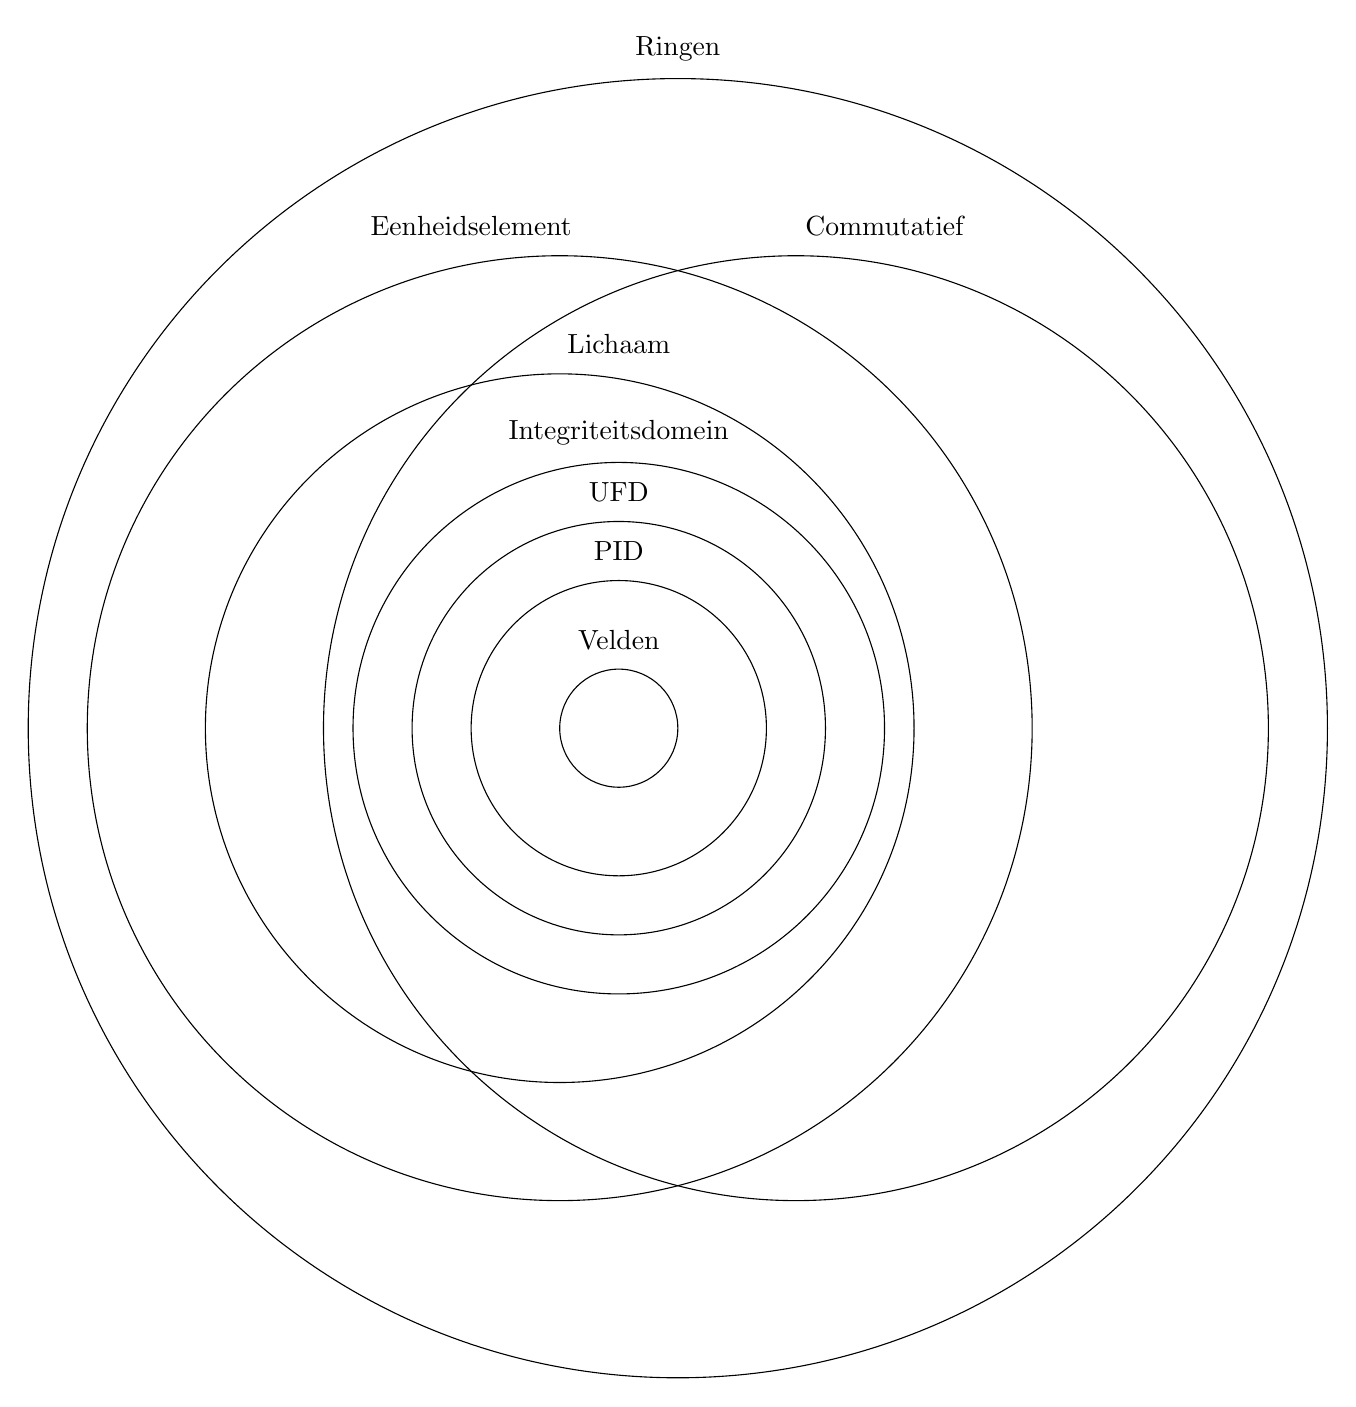
\begin{tikzpicture}[scale=1.5]
    \draw (0,0) circle (5.5cm);
    \draw (0,5.75) node {Ringen};
    \draw (-1,0) circle (4cm);
    \draw (-1.75,4.25) node {Eenheidselement};
    \draw (1,0) circle (4cm);
    \draw (1.75,4.25) node {Commutatief};
    \draw (-1,0) circle (3cm);
    \draw (-0.5,3.25) node {Lichaam};
    \draw (-.5,0) circle (2.25cm);
    \draw (-.5,2.5) node {Integriteitsdomein};
    \draw (-.5,0) circle (1.75cm);
    \draw (-.5,2) node {UFD};
    \draw (-.5,0) circle (1.25cm);
    \draw (-.5,1.5) node {PID};
    \draw (-.5,0) circle (0.5cm);
    \draw (-.5,0.75) node {Velden};
  \end{tikzpicture}
  \caption{Ringen}
  \label{fig:ringen}  
\end{figure}


\end{document}






